\section{Технический проект}
\subsection{Общая характеристика организации решения задачи}

Необходимо спроектировать и разработать сайт, который должен способствовать упрощению реализации цифровых предметов внутри игры «Stay Out».

Веб-сайт представляет собой набор взаимосвязанных электронных страниц, объединенных в логическую структуру и содержащих различные виды контента: текст, графику и мультимедийные элементы. Сайт разработан с использованием таких технологий, как HTML, CSS и JavaScript.

Разрабатываемый веб-сайт будет предоставлять пользователям возможность создания учетных записей, выставления и поиска внутриигровых ценностей, а также обмена ими с другими игроками. Он будет обеспечивать удобный интерфейс для взаимодействия между игроками, обеспечивая прозрачность и безопасность сделок.

\subsection{Обоснование выбора технологии проектирования}

Используемые для создания программно-информационной системы языки и технологии отвечают современным практикам разработки, позволяют достичь высокой производительности и отказоустойчивости программы.

\subsubsection{Описание используемых технологий и языков программирования}

В процессе разработки web-сайта используются программные средства и языки программирования. Каждое программное средство и каждый язык программирования применяется для круга задач, при решении которых они необходимы.

\subsubsection{Язык программирования JavaScript}

JavaScript - это интерпретируемый, объектно-ориентированный язык программирования, который широко используется для создания интерактивных и динамических веб-сайтов. Благодаря своей многофункциональности, JavaScript является одним из самых популярных языков программирования в мире веб-разработки.

В отличие от многих других языков программирования, JavaScript выполняется непосредственно в веб-браузере пользователя. Это позволяет ему взаимодействовать с элементами HTML страницы, управлять их содержимым, изменять стили, реагировать на пользовательские действия и многое другое, что делает веб-страницы более интерактивными и динамичными.

JavaScript широко используется для разработки различных веб-приложений, таких как интерфейсы пользователя, игры, анимации, формы обратной связи, веб-сервисы и многое другое. Благодаря своей популярности и гибкости, JavaScript также стал широко используемым для разработки серверной стороны приложений с использованием платформы Node.js.

Язык JavaScript имеет динамическую типизацию данных, что означает, что переменные не требуют явного объявления типа данных, и их тип может изменяться в процессе выполнения программы. Это делает JavaScript гибким и удобным для быстрой разработки прототипов и простых скриптов.

Важно отметить, что JavaScript не следует путать с языком Java, несмотря на сходство в названиях. JavaScript и Java - это разные языки программирования с разными синтаксисами, целями и областями применения. JavaScript был создан компанией Netscape в начале 1990-х годов и был изначально разработан для управления взаимодействием с пользователем на веб-страницах.

На сегодняшний день JavaScript является основным инструментом для создания интерактивных элементов на веб-страницах, таких как всплывающие окна, обновление данных без перезагрузки страницы (через AJAX), обработка событий от пользователя и многие другие. Современные фреймворки и библиотеки, такие как React, Angular и Vue.js, значительно упрощают и ускоряют процесс разработки сложных веб-приложений, предоставляя разработчикам мощные инструменты для создания высококачественных интерфейсов.

Кроме того, с развитием технологий JavaScript начал использоваться не только на стороне клиента, но и на стороне сервера. Платформа Node.js позволяет выполнять JavaScript код на сервере, что открывает новые возможности для создания масштабируемых и высокопроизводительных серверных приложений. Это делает JavaScript универсальным языком программирования, применимым как для клиентской, так и для серверной части веб-разработки.

\subsubsection{Библиотека React JS}

React -- это библиотека JavaScript с открытым кодом для создания внешних пользовательских интерфейсов. В отличие от других библиотек JavaScript, предоставляющих полноценную платформу приложений, React ориентируется исключительно на создание представлений приложений через инкапсулированные единицы (называются компонентами), которые сохраняют состояние и генерируют элементы пользовательского интерфейса. В React свойства передаются от родительских компонентов к дочерним. Компоненты получают свойства неизменяемых значений, из-за чего компонент не может напрямую изменять свойства, но может вызывать изменения через callback-функции.

\subsubsection{Фреймворк JS Express}

Express -- это фреймворк, написанный на языке JavaScript, который применяется в разработке бизнес-логики мобильных приложений и сайтов. Поскольку пользовательская часть сайтов работает исключительно на JavaScript, использование Express в качестве фреймворка позволяет задействовать JavaScript в пользовательской и серверной части веб-приложения.

\subsubsection{PostgreSQL}

PostgreSQL -- это объектно-реляционная система управления базами данных, основанная на POSTGRES - программе, разработанной на факультете компьютерных наук Калифорнийского университета в Беркли. У нее множество преимуществ, очень важным из которых является возможность установить СУБД на любую операционную систему, к тому же она бесплатная, что на том же MacOS является довольно важным критерием.

\subsubsection{Архитектура программной системы}

Разрабатываемая программная система основывается на клиент-серверной модели, которая является широко используемой парадигмой для разработки распределенных приложений. Эта модель позволяет распределять задачи и ответственность между несколькими компонентами, обеспечивая гибкость, масштабируемость и упрощение обслуживания. Клиентская часть системы является интерфейсом, с которым взаимодействует пользователь. Клиент выполняет функции отображения данных и приема ввода от пользователя. Серверная часть системы является компонентом, который обрабатывает запросы от клиентов, выполняет основную бизнес-логику и управляет данными. Сервер может быть размещен на мощных вычислительных платформах, обеспечивающих высокую производительность и надежность.

\subsection{Диаграмма компонентов}

Диаграмма компонентов является важным инструментом для описания физического представления разрабатываемой системы. Она позволяет разработчикам определить архитектуру системы, выявив взаимосвязи и зависимости между программными компонентами, включая как исходный, так и исполняемый код.

Основными элементами диаграммы компонентов являются компоненты, интерфейсы и зависимости между ними. Компоненты представляют собой логические единицы функциональности системы, которые могут быть как отдельными приложениями, так и более крупными модулями или сервисами.

\begin{figure}[h]
	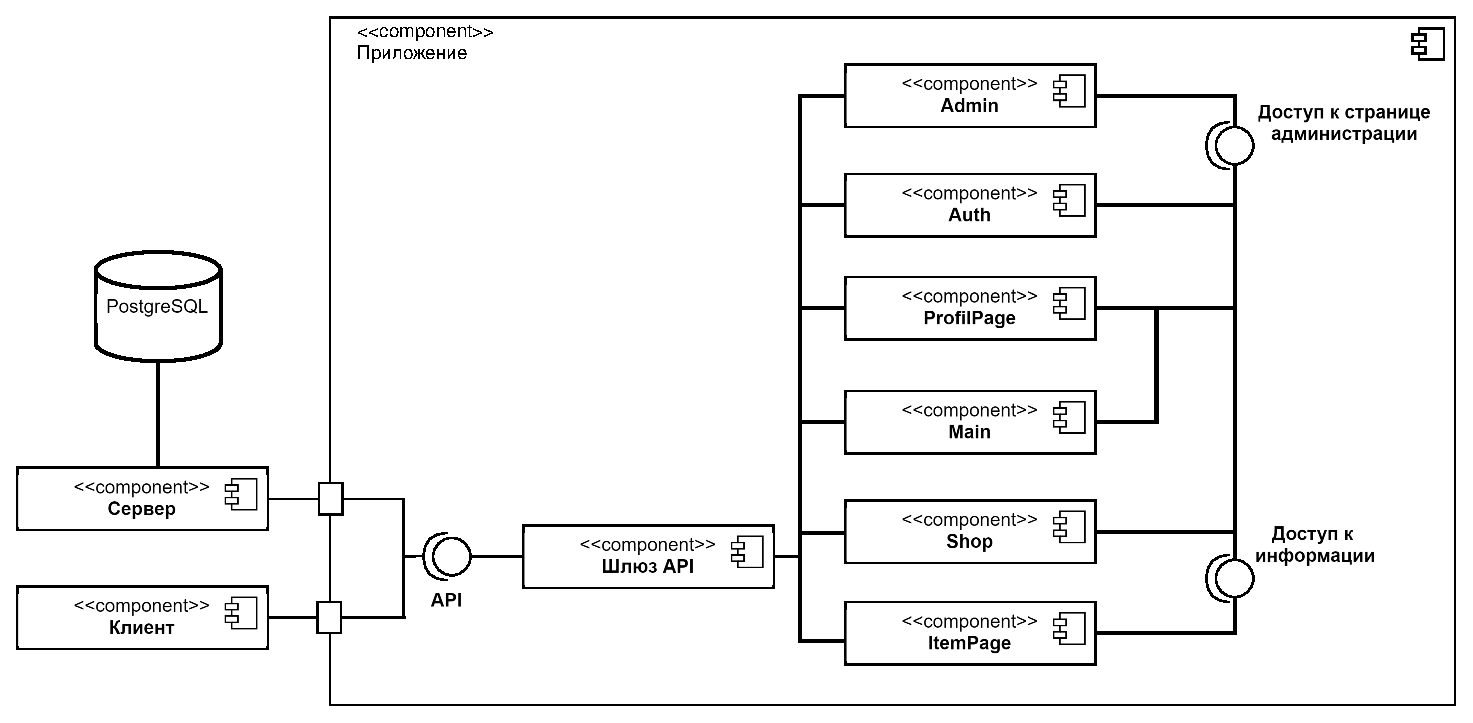
\includegraphics[width=1\linewidth]{images/diagcomp}
	\caption{Диаграмма компонентов}
	\label{fig:diagcomp}
\end{figure}

Интерфейсы определяют способы взаимодействия между компонентами, задавая набор методов, сообщений или протоколов, которыми компоненты обмениваются информацией.

Зависимости указывают на связи между компонентами, определяя порядок и направление потока данных или контроля между ними.

На рисунке \ref{fig:diagcomp} представлена диаграмма компонентов для проектируемой системы.

\subsection{Диаграмма размещения}

Диаграмма размещения используется для визуализации физического расположения компонентов программной системы на аппаратных платформах. Она является важным инструментом в процессе проектирования и реализации программного обеспечения, так как позволяет показать, как различные части системы будут распределены по различным узлам (например, серверам, компьютерам, сетевому оборудованию). Диаграмма размещения помогает архитекторам и разработчикам понять физическое развертывание системы, а также определить, какие узлы будут взаимодействовать друг с другом и каким образом.

На рисунке \ref{fig:diagrazm} представлена диаграмма размещения для проектируемой системы.

\vspace{-8mm} % чтобы убрать пустую строку, которая осталась после переноса рисунка на следующую страницу
\begin{figure}[h]
	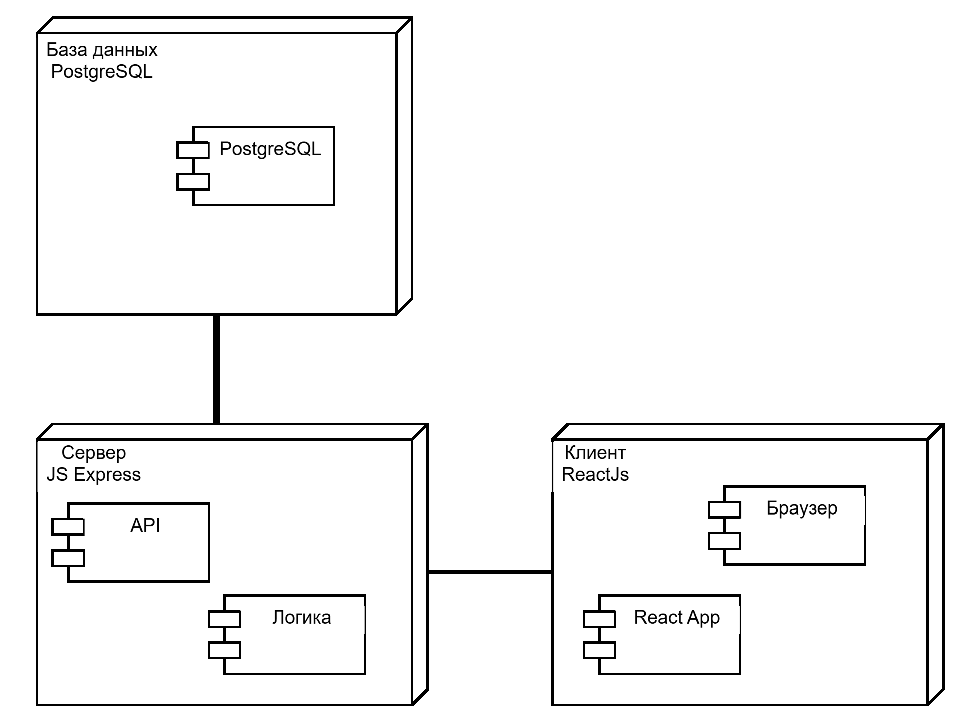
\includegraphics[width=0.5\linewidth]{images/diagrazm}
	\caption{Диаграмма размещения}
	\label{fig:diagrazm}
\end{figure}

\subsection{Конечные точки серверной части}

Для организации взаимодействия клиентской части с бизнес-логикой приложения были определены конечные точки. На рисунке \ref{fig:routes} представлена карта маршрутов, представляющее схематическое изображение конечных точек.

\begin{figure}
	\centering
	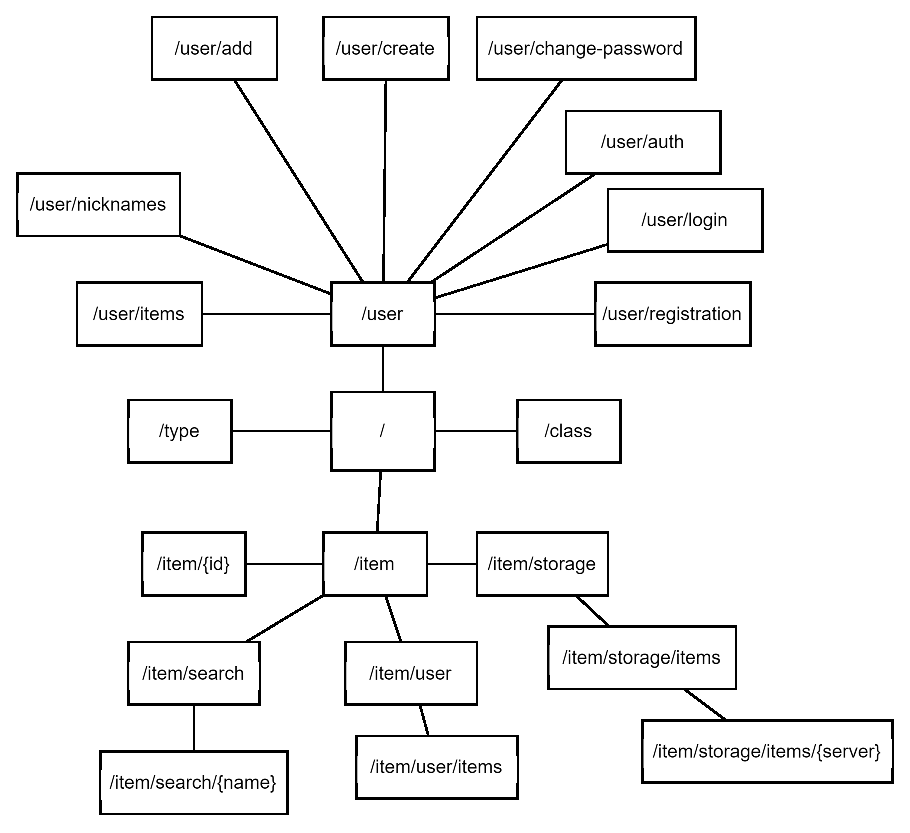
\includegraphics[width=0.7\linewidth]{images/routes}
	\caption{Карта маршрутов}
	\label{fig:routes}
\end{figure}

POST /user/registration - Регистрация нового пользователя.

POST /user/login - Вход пользователя в систему.

GET /user/auth - Проверка авторизации пользователя.

POST /user/change-password - Изменение пароля пользователя.

POST /user/create - Создание хранилища для пользователя.

POST /user/add - Добавление предмета в хранилище пользователя.

GET /user/items - Получение предметов из хранилища пользователя.

PUT /user/nicknames - Обновление никнеймов пользователя.

POST /class/ - Создание нового класса предмета.

GET /class/ - Получение всех классов предметов.

POST /type/ - Создание нового типа предмета.

GET /type/ - Получение всех типов предметов.

POST /item/ - Создание нового предмета.

GET /item/ - Получение всех предметов с возможностью фильтрации.

GET /item/:id - Получение конкретного предмета по его ID.

GET /item/search/:name - Поиск предметов по имени.

GET /item/storage/items/:server - Получение предметов из хранилища по серверу.

POST /item/storage/add - Добавление предмета в хранилище.

GET /item/user/items - Получение предметов пользователя.

DELETE /item/:id - Удаление предмета по его ID.

GET /item/ammo\_infos/:itemId - Получение информации о боеприпасах по ID предмета.

\subsection{Проект данных программной системы}

Согласно требованиям технического задания, веб-сайт должен взаимодействовать с двумя базами данных.

На серверной стороне предполагается использование PostgreSQL, реляционной базы данных, которая обеспечивает хранение структурированных данных.

Для веб-сайта предусмотрено использование локального хранилища localStorage для хранения JWT токена, что позволяет сайту сохранять информацию о сессии пользователя между сеансами.

Реляционные базы данных, такие как PostgreSQL, используют таблицы для хранения данных в структурированном формате и оперируют ими с помощью SQL. Этот подход обеспечивает надежность и консистентность данных.

Использование localStorage для хранения JWT токена позволяет сайту сохранять и использовать информацию о пользовательской сессии без необходимости подключения к сети, что улучшает пользовательский опыт и обеспечивает безопасность данных.

\subsection{Описание сущностей серверной части}

В состав сущности "<Пользователь"> можно включить атрибуты, представленные в таблице \ref{news:table}.

\begin{xltabular}{\textwidth}{|l|l|p{1.7cm}|X|}
	\caption{Атрибуты сущности "<Пользователь">\label{news:table}}\\ \hline
	\centrow Поле & \centrow Тип & \centrow Обяза\-тельное & \centrow Описание \\ \hline
	\thead{1} & \thead{2} & \centrow 3 & \centrow 4 \\ \hline
	\endfirsthead
	\continuecaption{Продолжение таблицы \ref{news:table}}
	\thead{1} & \thead{2} & \centrow 3 & \centrow 4 \\ \hline
	\finishhead
	id & ObjectId & true & Уникальный идентификатор \\ \hline 
	email & String & true & Почта \\ \hline 
	login & String & true & Псевдоним \\ \hline
	password & String & true & Пароль \\ \hline 
	role & String & true & Привилегия \\ \hline 
	status & String & true & Статус \\ \hline 
\end{xltabular}

В состав сущности "<Предметы"> можно включить атрибуты, представленные в таблице \ref{proda:table}.

\begin{xltabular}{\textwidth}{|R|C{2.5cm}|l|T|}
	\caption{Атрибуты  сущности "<Предметы"> с использованием различных типов столбцов и многострочным заголовком\label{proda:table}}\\ \hline
	\centrow Поле & \centrow Тип & \centrow Обязательное & \centrow Описание \\ \hline
	\centrow 1 & \centrow 2 & \thead{3} & \centrow 4 \\ \hline
	\endfirsthead
	\continuecaption{Продолжение таблицы \ref{proda:table}}
	\centrow 1 & \centrow 2 & \thead{3} & \centrow 4 \\ \hline
	\finishhead
	id & ObjectId & true & Уникальный идентификатор \\ \hline 
	name & String & true & Название \\ \hline 
	description & String & false & Описание \\ \hline 
	img & String & true & Путь до изображения \\ \hline 
	weight & String & true & Вес \\ \hline 
	level & String & true & Уровень \\ \hline 
\end{xltabular}

В состав сущности "<Тип"> можно включить атрибуты, представленные в таблице \ref{prod1:table}.

\begin{xltabular}{\textwidth}{|R|C{2.5cm}|l|T|}
	\caption{Атрибуты  сущности "<Тип"> с использованием различных типов столбцов и многострочным заголовком\label{prod1:table}}\\ \hline
	\centrow Поле & \centrow Тип & \centrow Обязательное & \centrow Описание \\ \hline
	\centrow 1 & \centrow 2 & \thead{3} & \centrow 4 \\ \hline
	\endfirsthead
	\continuecaption{Продолжение таблицы \ref{prod1:table}}
	\centrow 1 & \centrow 2 & \thead{3} & \centrow 4 \\ \hline
	\finishhead
	id & ObjectId & true & Уникальный идентификатор \\ \hline 
	name & String & true & Название \\ \hline 
	img & String & true & Путь до изображения \\ \hline 
\end{xltabular}

В состав сущности "<Класс"> можно включить атрибуты, представленные в таблице \ref{prod2:table}.

\begin{xltabular}{\textwidth}{|R|C{2.5cm}|l|T|}
	\caption{Атрибуты  сущности "<Класс"> с использованием различных типов столбцов и многострочным заголовком\label{prod2:table}}\\ \hline
	\centrow Поле & \centrow Тип & \centrow Обязательное & \centrow Описание \\ \hline
	\centrow 1 & \centrow 2 & \thead{3} & \centrow 4 \\ \hline
	\endfirsthead
	\continuecaption{Продолжение таблицы \ref{prod2:table}}
	\centrow 1 & \centrow 2 & \thead{3} & \centrow 4 \\ \hline
	\finishhead
	id & ObjectId & true & Уникальный идентификатор \\ \hline 
	name & String & true & Название \\ \hline 
	img & String & true & Путь до изображения \\ \hline 
\end{xltabular}

В состав сущности "<Экипировка"> можно включить атрибуты, представленные в таблице \ref{prod3:table}.

\begin{xltabular}{\textwidth}{|R|C{2.5cm}|l|T|}
	\caption{Атрибуты  сущности "<Экипировка"> с использованием различных типов столбцов и многострочным заголовком\label{prod3:table}}\\ \hline
	\centrow Поле & \centrow Тип & \centrow Обязательное & \centrow Описание \\ \hline
	\centrow 1 & \centrow 2 & \thead{3} & \centrow 4 \\ \hline
	\endfirsthead
	\continuecaption{Продолжение таблицы \ref{prod3:table}}
	\centrow 1 & \centrow 2 & \thead{3} & \centrow 4 \\ \hline
	\finishhead
	id & ObjectId & true & Уникальный идентификатор \\ \hline 
	lifting\_capacity & String & true & Грузоподъемность \\ \hline 
	melee & String & true & Рукопашная \\ \hline 
	explosion & String & true & Взрыв \\ \hline
	electric & String & true & Электрическое \\ \hline 
	infrared & String & true & Инфракрасное \\ \hline 
	radiation & String & true & Радиация \\ \hline 
	biological & String & true & Биологическое \\ \hline 
	frostbite & String & true & Обморожение \\ \hline 
	state & String & true & Состояние \\ \hline 
\end{xltabular}

В состав сущности "<Патроны"> можно включить атрибуты, представленные в таблице \ref{prod4:table}.

\begin{xltabular}{\textwidth}{|R|C{2.5cm}|l|T|}
	\caption{Атрибуты  сущности "<Патроны"> с использованием различных типов столбцов и многострочным заголовком\label{prod4:table}}\\ \hline
	\centrow Поле & \centrow Тип & \centrow Обязательное & \centrow Описание \\ \hline
	\centrow 1 & \centrow 2 & \thead{3} & \centrow 4 \\ \hline
	\endfirsthead
	\continuecaption{Продолжение таблицы \ref{prod4:table}}
	\centrow 1 & \centrow 2 & \thead{3} & \centrow 4 \\ \hline
	\finishhead
	id & ObjectId & true & Уникальный идентификатор \\ \hline 
	type\_ammo & String & true & Тип \\ \hline 
	breaking\_throught & String & true & Пробитие \\ \hline 
	damage & String & true & Урон \\ \hline 
\end{xltabular}

В состав сущности "<Оружие"> можно включить атрибуты, представленные в таблице \ref{prod5:table}.

\begin{xltabular}{\textwidth}{|R|C{2.5cm}|l|T|}
	\caption{Атрибуты  сущности "<Оружие"> с использованием различных типов столбцов и многострочным заголовком\label{prod5:table}}\\ \hline
	\centrow Поле & \centrow Тип & \centrow Обязательное & \centrow Описание \\ \hline
	\centrow 1 & \centrow 2 & \thead{3} & \centrow 4 \\ \hline
	\endfirsthead
	\continuecaption{Продолжение таблицы \ref{prod5:table}}
	\centrow 1 & \centrow 2 & \thead{3} & \centrow 4 \\ \hline
	\finishhead
	id & ObjectId & true & Уникальный идентификатор \\ \hline 
	moa & String & true & Угловая минута \\ \hline 
	rate\_of\_fire & String & true & Темп \\ \hline 
	breaking\_throught & String & true & Пробитие \\ \hline 
	strength & String & true & Прочность \\ \hline 
	recoil & String & true & Отдача \\ \hline 
	handing & String & true & Качание \\ \hline 
	rocw & String & true & Отказ от состояния \\ \hline 
	no\_pollutin & String & true & Отказ от загрязнения \\ \hline 
	type\_ammo & String & true & Тип патрона \\ \hline 
\end{xltabular}

В состав сущности "<Гранаты"> можно включить атрибуты, представленные в таблице \ref{prod6:table}.

\begin{xltabular}{\textwidth}{|R|C{2.5cm}|l|T|}
	\caption{Атрибуты  сущности "<Гранаты"> с использованием различных типов столбцов и многострочным заголовком\label{prod6:table}}\\ \hline
	\centrow Поле & \centrow Тип & \centrow Обязательное & \centrow Описание \\ \hline
	\centrow 1 & \centrow 2 & \thead{3} & \centrow 4 \\ \hline
	\endfirsthead
	\continuecaption{Продолжение таблицы \ref{prod6:table}}
	\centrow 1 & \centrow 2 & \thead{3} & \centrow 4 \\ \hline
	\finishhead
	id & ObjectId & true & Уникальный идентификатор \\ \hline 
	number\_of\_fragments & String & true & Количество осколков \\ \hline 
	shock\_wave\_radius & String & true & Радиус взрыва \\ \hline 
\end{xltabular}

В системе предусмотрен внутренний механизм связи между разделами и элементами информационных блоков, что обеспечивает эффективную организацию данных без необходимости введения дополнительных идентификаторов при реализации связей между сущностями.

Каждая сущность в системе представлена экземпляром информационного блока, который содержит элементы, отражающие конкретные атрибуты или характеристики данной сущности. Поля и свойства элементов информационных блоков служат для описания атрибутов сущности.

Благодаря этому подходу, данные о сущностях хранятся и управляются структурированно и легко доступны для обработки. Экземпляры сущностей, представленные элементами информационных блоков, обеспечивают гибкость в управлении данными, позволяя эффективно адаптировать информационную структуру системы к различным потребностям и изменениям в бизнес-логике.

Такой подход минимизирует необходимость введения дополнительных идентификаторов или средств для организации связей между сущностями, упрощая процесс разработки и поддержки системы. Кроме того, он способствует повышению производительности и надежности обработки данных, так как предусматривает оптимальное использование внутренних механизмов управления информацией.

\subsection{Проектирование пользовательского интерфейса}

На основе требований к пользовательскому интерфейсу, представленных в пункте 2.3.3 технического задания, был разработан графический интерфейс для взаимодействия с приложением. Для стилизации некоторых компонентов использовался CSS 3. Для разработки интерфейса использовалась библиотека React вместе с библиотекой React-компонентов React-Bootstrap. На представленных ниже рисунках числами обозначены элементы графического интерфейса. На рисунке \ref{fig:regmaket} представлен макет страницы регистрации пользователя. Страница регистрации содержит следующие элементы:

\begin{enumerate}
	\item Форма регистрации.
	\item Поле ввода электронной почты.
	\item Поле ввода пароля.
	\item Ссылка на форму авторизации.
	\item Кнопка подтверждения формы.
\end{enumerate}

\begin{figure}
	\centering
	\includegraphics[width=0.7\linewidth]{images/reg_maket}
	\caption{Макет страницы регистрации}
	\label{fig:regmaket}
\end{figure}

На рисунке \ref{fig:logmaket} представлен макет страницы авторизации. Страница авторизации содержит следующие элементы:

\begin{enumerate}
	\item Форма авторизации.
	\item Поле ввода электронной почты.
	\item Поле ввода пароля.
	\item Ссылка на форму регистрации.
	\item Кнопка подтверждения формы.
\end{enumerate}

\begin{figure}
	\centering
	\includegraphics[width=0.7\linewidth]{images/log_maket}
	\caption{Макет страницы авторизации}
	\label{fig:logmaket}
\end{figure}

На рисунке \ref{fig:mainmaket} представлен макет главной страницы. Главная страница содержит следующие элементы:

\begin{enumerate}
	\item Ссылка на главную страницу.
	\item Кнопка вызова формы выбора сервера.
	\item Кнопка перехода на страницу администрации.
	\item Кнопка перехода в профиль.
\end{enumerate}

\begin{figure}
	\centering
	\includegraphics[width=0.7\linewidth]{images/main_maket}
	\caption{Макет главной страницы}
	\label{fig:mainmaket}
\end{figure}

На рисунке \ref{fig:shopmaket} представлен макет страницы маркетплейса. Страница маркетплейса содержит следующие элементы:

\begin{enumerate}
	\item Ссылка на главную страницу.
	\item Тип предмета.
	\item Класс предмета.
	\item Форма предмета.
	\item Изображение предмета.
	\item Никнейм игрового персонажа.
	\item Характеристики предмета.
	\item Кнопка покупки предмета.
	\item Кнопка перехода на страницу администрации.
	\item Кнопка перехода в профиль.
	\item Отображение выбранной страницы.
	\item Кнопка выставления предмета на продажу.
\end{enumerate}

\begin{figure}
	\centering
	\includegraphics[width=0.7\linewidth]{images/shop_maket}
	\caption{Макет страницы магазина}
	\label{fig:shopmaket}
\end{figure}

